\subsection{Merge-Sort Results:}

Test of Merge-Sort Algorithm. The program will plot the {\bfseries\itshape time} that the algorithm takes to sort a 'list' of size {\bfseries\itshape n = 6}.

\begin{figure}[H]
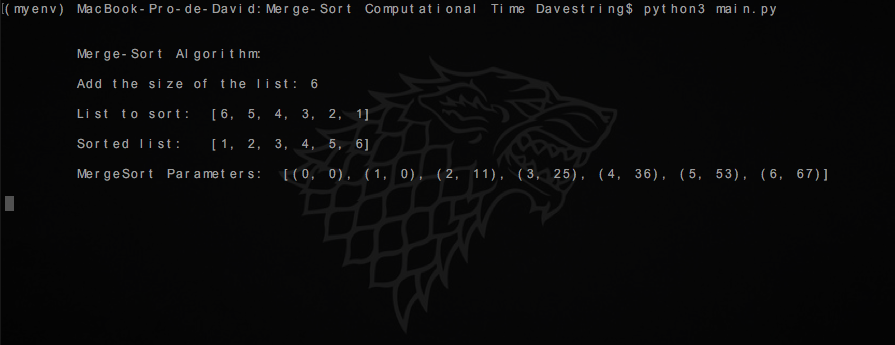
\includegraphics[scale=.5]{console1.png}
\centering \linebreak \linebreak Figure 5.1.0: Console output of Merge-Sort algorithm.
\end{figure} 

\begin{multicols}{2}
\begin{figure}[H]
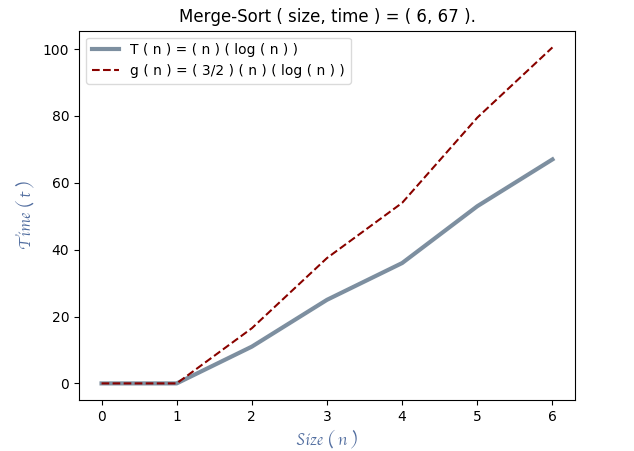
\includegraphics[scale=.45]{plot1.png}
\centering \linebreak \linebreak Figure 5.1.1: Plot of Figure 4.1.0.
\end{figure} 

\begin{center}
\begin{itemize}
\end{itemize}
{\Large
\begin{tabular}[.5cm]{c c c }
\toprule
Size ( n ) & Time ( t ) \\
\midrule
0 & 0 \\
\cmidrule{1-2}
1 & 0 \\
\cmidrule{1-2}
2 & 11 \\
\cmidrule{1-2}
3 & 25 \\
\cmidrule{1-2}
4 & 36 \\
\cmidrule{1-2}
5 & 53 \\
\cmidrule{1-2}
6 & 67 \\
\bottomrule
\linebreak
\end{tabular}}
\linebreak \linebreak Table 1: Plot points of Figure 4.1.1.
\end{center}
\end{multicols} \hfill

{\bfseries\itshape\color{armygreen}{Observation:}} {\itshape\color{armygreen}{Remember that in {\bfseries main.py} the program split the 'list' into sublists {\bfseries $B_{i}$} and calculates the computational time that takes to sort each one until {\bfseries $B_{i}$ = A}, The column {\bfseries Size} in the table it's the length of this {\bfseries $B_{i}$} lists.}}  \hfill \break


{\bfseries\itshape\color{armygreen}{Observation:}} {\itshape\color{armygreen}{The plot has two curves, the blue one it’s the computation time of our algorithm: \linebreak {\bfseries T ( n ) = ( n ) ( log ( n ) )}, and the red one it's a proposed function {\bfseries g ( n ) = ( 3/2 ) ( n ) ( log ( n ) )} \linebreak where {\bfseries T( n ) $\in\ \theta$ ( g ( n ) )}.}} \hfill \break

{\bfseries\itshape\color{armygreen}{Observation:}} {\itshape\color{armygreen}{For this example we are analyzing a worst case.}} 

\pagebreak